%!TEX TS-program = xelatex
%!TEX encoding = UTF-8 Unicode

\def \papersize {a4paper}
\documentclass[12pt,\papersize]{extarticle}
% extarticle is like article but can handle 8pt, 9pt, 10pt, 11pt, 12pt, 14pt, 17pt, and 20pt text

\def \ititle {How to Construct a Minimal Theory of Mind}
\def \isubtitle {}
\def \iauthor {Stephen A. Butterfill \& Ian A. Apperly}
\def \iemail{s.butterfill@warwick.ac.uk}
%for anonymous submisison
%\def \iauthor {}
%\def \iemail{}
%\date{}

%!TEX TS-program = xelatex
%!TEX encoding = UTF-8 Unicode

\title{\ititle\\\isubtitle}
\author{\iauthor\\<{\iemail}>}

\usepackage[\papersize]{geometry} % see geometry.pdf
\geometry{twoside=false}
\geometry{headsep=2em} %keep running header away from text
\geometry{footskip=1cm} %keep page numbers away from text
\geometry{top=3cm} %increase to 3.5 if use header
\geometry{left=4cm} %increase to 3.5 if use header
\geometry{right=4cm} %increase to 3.5 if use header
\geometry{textheight=22cm}

%non-xelatex
%\usepackage[T1]{fontenc}
%\usepackage{tgpagella}

%for underline
\usepackage[normalem]{ulem}

%get the font here:
% http://scripts.sil.org/CharisSILfont

\usepackage{fontspec,xunicode}
%nb do not explicitly use package xltxtra because this introduces bugs with footnote superscripting  -- perhaps because fontspec is supposed to include it anyway.
%UPDATE:  "You need to use the no-sscript option in xltxtra: \usepackage[no-sscript]{xltxtra}, this is explained in the documentation of xltxtra.  The issue is that Sabon does not contain true superscript glyphs for every character and the no-sscript option will instead use scaled regular glyphs, which is typographically inferior, but there is no other option available when using Sabon." --- http://groups.google.com/group/comp.text.tex/browse_thread/thread/19de95be2daacade
\defaultfontfeatures{Mapping=tex-text}
%\setromanfont[Mapping=tex-text]{Charis SIL} %i.e. palatino
%\setromanfont[Mapping=tex-text]{Sabon LT Std} 
%\setromanfont[Mapping=tex-text]{Dante MT Std} 
%\setromanfont[Mapping=tex-text,Ligatures={Common}]{Hoefler Text} %comes with osx
\setromanfont[Mapping=tex-text]{Linux Libertine O} 
\setsansfont[Mapping=tex-text]{Linux Biolinum O} 
\setmonofont[Scale=MatchLowercase]{Andale Mono}


%hyperlinks and pdf metadata
%TODO avoid duplication of title & author
\usepackage{hyperref}
\hypersetup{pdfborder={0 0 0}}
\hypersetup{pdfauthor={\iauthor}}
\hypersetup{pdftitle={\ititle\isubtitle}}


%handles references to labels (e.g. sections) nicely
\usepackage{varioref}

%line spacing
\usepackage{setspace}
%\onehalfspacing
%\doublespacing
\singlespacing

\usepackage{natbib}
%\usepackage[longnamesfirst]{natbib}
\setcitestyle{aysep={}}  %philosophy style: no comma between author & year

%enable notes in right margin, defaults to ugly orange boxes TODO fix
%\usepackage[textwidth=5cm]{todonotes}

%for comments
\usepackage{verbatim}

%footnotes
\usepackage[hang]{footmisc}
\setlength{\footnotemargin}{1em}
\setlength{\footnotesep}{1em}
\footnotesep 2em

%tables
\usepackage{booktabs}
\usepackage{ctable}

%section headings
\usepackage[sf]{titlesec}
%\titlespacing*{\section}{0pt}{*3}{*0.5} %reduce vertical space after header
%large headings:
%\titleformat{\section}{\LARGE\sffamily}{\thesection.}{1em}{} 
\titlelabel{\thetitle.\quad}

%captions
\usepackage[font={small,sf}, margin=0.75cm]{caption}

%lists
\usepackage{enumitem}
\newenvironment{idescription}
{ 	
	% begin code
	\begin{description}[
		labelindent=1.5\parindent,
		leftmargin=2.5\parindent
	]
}
{ 
	%end code
	\end{description}
}


%title
\usepackage{titling}
\pretitle{
	\begin{center}
	\sffamily
	\Huge
} 
\posttitle{
	\par
	\end{center}
	\vskip 0.5em
} 
\preauthor{
	\begin{center}
	\normalsize
	\lineskip 0.5em
	\begin{tabular}[t]{c}
} 
\postauthor{
	\end{tabular}
	\par
	\end{center}
}
\predate{
	\begin{center}
	\normalsize
} 
\postdate{
	\par
	\end{center}
}



%avoid overhang
\tolerance=5000


\begin{document}

\setlength\footnotesep{1em}

\bibliographystyle{newapa} %apalike

%these two lines are for anonymous submission --- they remove author and date
%but don't forget to remove defs above as well --- otherwise it will be in the metadata
%\author{}
%\date{}


\maketitle
%\tableofcontents

\begin{abstract}
\noindent
What could someone represent that would enable her to track, at least within limits, perceptions, knowledge states and beliefs including false beliefs? 
An obvious possibility is that she might represent these very propositional attitudes as such.
It is sometimes tacitly or explicitly assumed that this is the only possible answer.
However we argue that several recent discoveries in developmental, cognitive, and comparative psychology indicate the need for other, less obvious possibilities.
Our aim is to meet this need by describing the construction of a minimal theory of mind.  
Minimal theory of mind is rich enough to explain systematic success on tasks held to be acid tests for theory of mind cognition including many false belief tasks.  
It is also extensible in ways that can explain a wide range of findings from non-human animals and human infants that are sometimes presented as evidence for full-blown theory of mind cognition.  
Yet minimal theory of mind does not require representing propositional attitudes, or any other kind of representation, as such.
Minimal theory of mind may be what enables those with limited cognitive resources or little conceptual sophistication, such as infants, chimpanzees, scrub-jays and human adults under load, able to track, within limits, facts about perceptions and beliefs.

\ 

\noindent
\textbf{Keywords:}
Theory of Mind, False Belief, belief, perception, development, comparative
\end{abstract}



\section{Introduction}
What could someone represent that would enable her to track, at least within limits, perceptions, knowledge states and beliefs including false beliefs? 
One answer is obvious: she might track these things by virtue of representing them as such, that is, by representing perceptions, beliefs, and other propositional attitudes as such.
Our aim in what follows is to identify another, less obvious answer.
There is a form of cognition---minimal theory of mind---which does not involve representing propositional attitudes as such but does involve representing simpler, relational mental states which could, within limits, enable one to track propositional attitudes such as beliefs.
Minimal theory of mind 
is  rich enough to enable systematic success on tasks held to be acid tests for theory of mind cognition including many false belief tasks.
As we will explain, this has consequences 
for interpreting a range of findings concerning infants', adults' and nonhumans' performances on theory of mind tasks.
It may help us to understand what enables those with limited cognitive resources or little conceptual sophistication, such as infants, chimpanzees, scrub-jays and human adults under load, to track, within limits, facts about perceptions and beliefs.

In this section we defend explain our question; in the next sections we introduce the findings which motivate facing it before starting to answer it in the fourth section.

Some may find our question initially incomprehensible.
Could abilities to track false beliefs (say) really involve anything other than representing false beliefs?
To see the possibility of a positive answer it may help to consider a non-mental analogy.
What could someone represent that would enable her to track, at least within limits, the toxicity of potential food items?
Here the most straightforward answer (she could represent their toxicity) is clearly not the only one.
After all, someone might track toxicity by representing odours or by representing visual features associated with putrefaction, say.
Suppose Sin\'ead has no conception of toxins but represents the odours of food items and 
treats those with foul odours as dangerous to eat,
so that she would not normally offer them to friends or family
nor conceal them from competitors.
This brings nutritional and competitive benefits obtaining which depends on facts about toxicity.
If Sin\'ead tends to behave in this way because of these benefits, 
representing odours enables her to track, in a limited but useful range of cases,  toxicity.
Our question, put very roughly, is whether   belief has something like an odour.

To make the question more precise it is useful to distinguish 
theory of mind abilities from theory of mind cognition.  
A  \textit{theory of mind ability} 
	\label{df:tom_ability}
is an ability that exists in part because exercising it brings benefits obtaining which depends on exploiting or influencing facts about others’ mental states.
To illustrate,
suppose that Hannah is able to discern whether another's eyes are in view,
that Hannah exercises this ability to escape detection while stealing from others,
that Hannah's ability exists in part because it benefits her in this way,
and 
that Hannah's escaping detection depends on exploiting a fact about other's mental states (namely that they usually cannot  see Hannah's acts of theft when Hannah doesn't have their eyes in view).
Then Hannah has a theory of mind ability.
(This is not supposed to be a plausible, real-world example but only to illustrate what the definition requires.)
An ability to \textit{track} 
	\label{df:track} 
perceptions or beliefs (say) is a theory of mind ability which involves exploiting or influencing facts about these states.
By contrast, \textit{theory of mind cognition} 
	\label{df:tom_cognition}
involves representing mental states or processes as such.
And \textit{full-blown} theory of mind cognition involves  representing propositional attitudes such as beliefs, desires and intentions to construct reason-giving, causal explanations of action.  
The distinction between theory of mind abilities and theory of mind cognition matters because the facts about other minds which theory of mind abilities exploit are not necessarily the facts which are represented in theory of mind cognition.  
To return to the illustration, Hannah is able, within limits, to exploit facts about what others perceive without representing perceptions as such. 
She has a theory of mind ability while possibly lacking any theory of mind cognition.

It should be uncontroversial that some theory of mind abilities do not necessarily involve any theory of mind cognition at all. 
Our question concerns abilities to track what others perceive and believe, including their false beliefs; these have been central in psychological research.
Can anything less than full-blown theory of mind cognition  explain systematic success on a range of false belief tasks?
We do not aim to argue that someone could track beliefs, true and false, without any theory of mind cognition at all.
Our concern is rather with the construction of a minimal form of theory of mind cognition.
As we shall explain, minimal theory of mind does involve representing  belief-like  states, but it does not involve representing beliefs or other propositional attitudes as such.

The notion that some abilities to track perceptions, knowledge states or beliefs involve only theory of mind cognition which does not involve representing perceptions or beliefs as such is not entirely novel.
To mention only those we draw most directly on, Gomez (\citeyear[][p.\ 730]{en_1259}) has emphasized primitive intentional relations to objects established by gaze, O’Neil and Doherty have separately discussed a notion of engagement with objects (\citealp{en_1159, en_1140}), Call and Tomasello (\citeyear[][p.\ 58]{en_1669}) have suggested that chimpanzees track the `likely target' of others’ visual access and understand something about its effects on behaviour, and Whiten (\citeyear[]{en_1415, en_1416}) uses the notion of an `intervening variable' to explain primitive theory of mind notions.  These are illuminating ideas and what follows can be seen as an elaboration and partial synthesis of them.  
The result---minimal theory of mind---is unlike its precursors in that it is rich enough to explain systematic success on a range of false belief tasks.  Our approach is novel in this and others respects to which we return (in the Conclusion) after presenting the substance of our account.



%The notion that theory of mind cognition could involve representing non-propositional counterparts of belief 
%According to Davidson, 
%\begin{quote}
%`We are stuck with our two main ways of describing and explaining things, one which treats objects and events as mindless, and the other which treats objects and events as having propositional attitudes. I see no way of bridging the gap by introducing an intermediate vocabulary.' \citep[p.\ 697]{Davidson:2003bw}
%\end{quote}
%It may be tempting to dismiss this assertion on the grounds that we can readily describe an infant as excited by a clapping game, or as preferring one toy to another. 
%On the surface at least, these descriptions seem neither to involve propositional attitudes nor to involve treating the infant as mindless; it seems there are non-propositional forms of excitement and preference which are nevertheless mental states.
%
%Even so, Davidson is right that there is a genuine difficulty when it comes to understanding non-propositional counterparts of attitudes like belief and perception.  We cannot rely entirely on commonsense here because our commonsense concepts of perception, belief, intention and action exhibit a form of holism: we grasp them only if we understand their interdependent roles in reason explanations (Davidson 1995b, 1995a). 
%




\section{Motivation}
\label{sec:motivation}
Our question is theoretical: it concerns 
not what anyone does represent
but what someone could represent that would enable her, at least within limits, to track perceptions, knowledge states and beliefs.
The motivation for facing up to this question is, of course, partly empirical.

Consider ordinary adult humans.
Since they can represent beliefs and other propositional attitudes as such, 
it is natural to assume that such representations underpin their abilities to track perceptions and beliefs.
But is this natural assumption correct?

To see that it might not be, consider a further question.
Is tracking others' perceptions and beliefs automatic?
Roughly speaking,
a process is \emph{automatic} if whether it occurs is to a significant degree independent of its relevance to the particulars of the subject's motives and aims.
(Note that a process may occur spontaneously without thereby being automatic.)  
Some evidence suggests that, for ordinary adult humans, belief tracking is automatic.
For example,
\citet{kovacs_social_2010} asked adults to identify the location of a ball.
They found that adults were significantly slower to identify the ball's location when an onlooker had a false belief about the location of the ball,
even though the onlooker's belief was not relevant to the task at all.
Relatedly, \citet{Samson:2010jm} provide evidence that identifying what another perceives is automatic;  this finding is indirectly supported by  evidence that tracking others' perceptions is not disrupted by a secondary executive task \citep{qureshi:2010_executive}.
Taken together, these findings suggest that, at least in adults, tracking others' perceptions and beliefs is sometimes automatic.

But there is also a body of evidence supporting a different conclusion.
\citet{back:2010_apperly} found that subjects are significantly slower to answer an unexpected question about another's belief when that belief is false compared to when it is true \citep[see also][]{apperly:2006_belief}.
This suggests that, at least in adults, belief tracking is not automatic.
There is also evidence that, even in relatively simple situations, 
using facts about others' beliefs is not automatic \citep{Keysar:2003xu,apperly:2010_limits}.
The case for nonautomaticity is indirectly supported by evidence that tracking perceptions and beliefs---and even merely holding in mind what another believes, where no inference is required---involves a measurable processing cost  \citep{apperly:2008_back,apperly:2010_limits}, consumes attention and working memory in fully competent adults (\citealp{en_1698, lin:2010_reflexively, en_1547} experiments 4-5), may require inhibition \citep{bull:2008_role} and makes demands on executive function \citep{apperly:2004_frontal,samson:2005_seeing}.
These findings, taken together, suggest that tracking others' perceptions and beliefs is sometimes not automatic.

The question was whether, in adult humans,  tracking perception and belief is automatic.  
If we assume, further, that either all such processes are automatic or else none are, then the evidence creates a conflict.
This conflict  cannot easily be explained away by appeal to simple methodological factors or extraneous task demands.
For instance, it may be tempting to suppose that the conflict can be explained by distinguishing between linguistic and nonlinguistic tasks.  
But belief ascription may fail to be automatic even on some nonlinguistic tasks \citep[e.g.][]{apperly:2004_frontal}, and we know of no reason to assume that belief ascription could not be automatic on some linguistic theory of mind tasks (such as those where spontaneous tracking is already established, e.g.\ \citet{ferguson_listeners_2012}).

If the conflict is not a methodological artefact, how should we interpret the evidence?
Perhaps it should be taken at face value.
This means we must reject the assumption that tracking others' perceptions and beliefs is either always automatic or else always nonautomatic.
In other cases, such as number and causation, it is already quite widely accepted that, in adult humans, some abilities to track these things are automatic whereas others are not.\footnote{
On number: \citet{trick:1994_small};
on causation: \citet{Michotte:1946nz}, \citet{Scholl:2004dx}.
}
The evidence suggests that the same may be true for perception and belief.
In adult humans, some theory of mind abilities involve automatic processes whereas others depend on nonautomatic processes. 

A closely related view has already been elaborated and defended in more detail by
\citet[]{Apperly:2009ju},
although their argument complements ours by drawing  primarily on developmental and comparative research. 
According to them,
adults may enjoy efficient but inflexible forms of theory of mind cognition in addition to the full-blown form which involves representing beliefs and other propositional attitudes as such.
While aspects of this conjecture have already been tested \citep[]{Samson:2010jm, en_2397, surtees_direct_2011}, it raises two complementary questions (as Apperly \& Butterfill themselves note).  

First, why isn't tracking belief and perception always automatic?
Consider what is involved in representing beliefs and other propositional attitudes.
On any standard view, propositional attitudes form complex causal structures, have arbitrarily nestable contents, interact with each other in uncodifiably complex ways and are individuated by their causal and normative roles in explaining thoughts and actions \citep[]{en_809, en_249}.  
If anything should consume working memory and other scarce cognitive resources, it is surely representing states with this combination of properties.
So even without knowing in any detail how theory of mind cognition is implemented, it is plausible that some feature, or combination of features, of the propositional attitudes  makes full-blown theory of mind cognition demanding.%
\footnote{
Several hypotheses about which feature of the propositional attitudes explains why full-blown theory of mind cognition is cognitively and conceptually demanding have been defended \citep[e.g.][]{en_1263, en_634, en_1269, en_78, en_81, en_404, 	%en_687, %bibtex error authors and year too similar
	en_643, en_1130}.  
More than one feature may contribute. 
We are agnostic about which feature or features are to blame.
}  
%
A possible explanation, then, is this.
Tracking perception or belief is not always automatic because 
it sometimes involves representing propositional attitudes as such,
which typically or always places demands on working memory, attention and executive function  that are incompatible with automaticity.


Second, how could  tracking perceptions or beliefs ever be automatic?
If we assumed that such tracking always involved propositional attitudes as such, this question would present a puzzle.
For, as we saw, representing propositional attitudes as such generally places demands on working memory, attention and executive function that are incompatible with automaticity.
In some cases these demands might be overcome through automatization in something like the way that initially effortful numerical operations can through practice become automatic.\footnote{
On the automatization of simple sums, see \citet{lefevre:1988_cognitive}.
For the suggestion that something similar might happen concerning mental states, see \citet{Suddendorf:2003co}.
%which is also discussed by \citet[p.\ 961]{Apperly:2009ju}.
}
However, almost nothing is known about to what extent, if any, automatization occurs in theory of mind. 
And in any case automatization can only explain the automaticity of routine inferences.
So it is possible that automatization, although perhaps important, does not fully explain the automaticity of some of adult humans' perception- and belief-tracking abilities.
A full explanation may  depend on showing that tracking perceptions and beliefs can be done without  representing beliefs or other propositional attitudes as such.

This is a source motivation for our question about what someone could represent that would enable her to track perceptions and beliefs.
The existence of both automatic and nonautomatic tracking of perceptions and beliefs in human adults 
suggests (without decisively showing, of course), 
contrary to a natural assumption mentioned above,
that not all of their abilities to track perceptions and beliefs involve representing propositional attitudes as such.

\section{More motivation}
\label{sec:more_motivation} 
Further motivation for our question comes from evidence for theory of mind abilities in young children and infants.
Children in their second year use pointing to provide information to others \citep[]{en_1093} in ways that reflect a partner’s ignorance or knowledge \citep[]{en_1699}, as well as providing more information to ignorant than knowledgeable partners when making requests \citep[]{en_1140}.  One-year-old children also predict actions of agents with false beliefs about the locations of objects \citep[]{en_1092, en_1208} and choose different ways of interacting with others depending on whether their beliefs are true or false \citep[]{en_1783,Knudsen:2011fk,southgate:2010fb}.  And in much the way that irrelevant facts about the contents of others’ beliefs modulate adult subjects’ response times, such facts also affect how long 7-month-old infants look at some stimuli \citep[]{kovacs_social_2010}.

What do these infants and young children represent that enables them, within limits, to track others’ perceptions, knowledge states and beliefs?   
The most straightforward answer would be to suppose that they represent perceptions, knowledge states and beliefs as such \citep[e.g.][]{en_1138, en_1691}.  
But this answer faces several objections.  A body of evidence  suggests that representing beliefs requires conceptual sophistication, for it has a protracted developmental course stretching over several years \citep[]{en_87, en_89} and its acquisition is tied to the development of executive function \citep[]{en_410, en_1130} and language \citep[]{en_1209}.  Infants and young children are deficient in these.  
Development of reasoning about beliefs in humans may also be facilitated by explicit training \citep[]{en_85} and environmental factors such as siblings \citep[]{en_507, en_1299}.  
This is evidence that representations of belief in humans typically emerge from extensive participation in social interactions (as \citealp{en_1300} suggest).  
If any of this is right, we must reject the hypothesis that infants are representing beliefs or other propositional attitudes as such.

In principle an alternative would be to suppose that infants' and young children's abilities to track perceptions and beliefs 
do not involve any theory of mind cognition at all
but are instead based on 
representations of nonintentional behaviour only.
It is arguably possible in principle to explain some belief-tracking abilities by appeal to hypothetical behaviour reading capacities  \citep{perner:1988_developing,en_1168, en_1169}.
But there are several objections to the claim that the full range of even infants' abilities to track perceptions and beliefs could be explained in this way \citep{en_1691,Apperly:2009ju}.  
And what is is currently known about humans' actual behaviour reading capacities suggests that they are unlikely to explain systematic success on false belief tasks.%
\footnote{
Key studies include
	\citet{Newtson:1976ni}, 
	\citet{Byrne:1999jk},
	\citet{Baldwin:2001rs},
	\citet{Saylor:2007pj} and
	\citet{Baldwin:2008mw}.
} 
 
Here, then, is a second source of motivation for our question about what someone could represent that would enable her, within limits, to track perceptions and beliefs.
As we have seen, there are significant if not decisive objections to the two best developed conjectures about infant theory of mind abilities, the conjecture that these involve representing perceptions, knowledge states and beliefs as such and the conjecture that these involve representing nonintentional behaviour only.  
These objections, while not decisive, justify exploring alternatives.

Theory of mind abilities are not only found in humans.
For instance,
scrub-jays can selectively re-cache their food in ways that deprive competitors of knowledge of its location \citep{Clayton:2007fh}, and  chimpanzees can both select routes to approach food which conceal them from a competitor’s view \citep[]{en_1546} and also retrieve food using strategies that optimize their return given what a dominant competitor has seen \citep[]{en_1545}.  
There is debate about the cognitive underpinnings of these abilities. 
Some researchers argue that they may involve representations of nonintentional behaviour only,\footnote{
For example, on chimpanzees: 
	\citet{povinelli:2004vonk}; 
	\citet[pp.\ 364-5]{Vonk:2006cq}; and on scrub-jays and chimpanzees \citet{Penn:2007ey}.
} 
others that they involve representations of perceptions, knowledge states and other propositional attitudes.\footnote{
For example, on chimpanzees: \citet{Tomasello:2005ce,
			Call:2008di}; and on scrub-jays: 
			\citet[p.\ 73]{Emery:2007ze}.
}
If these arguments are not yet decisive
and if the available evidence does not already tightly constrain the space of admissible conjectures,
then the construction of a minimal theory of mind may also be relevant to these debates.
For the conjecture that minimal theory of mind explains chimpanzees' or scrub-jays' abilities to track perceptions or beliefs can be empirically distinguished from conjectures about representations of nonintentional behaviour only and from conjectures about representations of perceptions, knowledge states and beliefs (as we explain in section *** below).


%The construction of minimal theory of mind shows that there is a form of theory of mind cognition which does not involve representing beliefs or other propositional attitudes as such but is capable of explaining, within limits, systematic success on a range of false belief tasks.
%As we shall show,
%the conjecture that minimal theory of mind cognition underpins some abilities to track perceptions and belief in human adults and infants generates testable predictions that distinguish it from the alternatives.







\section{Minimal theory of mind}

In this section we begin with someone, call her Lucky, capable  of representing nonintentional behaviour only and ask what more is needed for minimal theory of mind cognition.  We describe Lucky’s progress with a series of principles. The principles are constructed in such a way that it would be coherent to suppose that Lucky has the abilities codified by the first \textit{n} principles only. They are not intended to represent a developmental or evolutionary progression.  The principles can also be extended to explain more sophisticated theory of mind abilities than those considered here.  We restrict ourselves to these five principles because they are sufficient to explain success on some false belief tasks.%
\footnote{
In standard false belief tasks, `[t]he subject is aware that he/she and another person [call him Maxi] witness a certain state of affairs x.  Then, in the absence of the other person the subject witnesses an unexpected change in the state of affairs from x to y' \citep[][p.\ 106]{en_89}.  The test concerns whether the subject realises that Maxi will falsely believe x to obtain.  In many cases the states of affairs, x and y, differ only with respect to the location of an object \citep[e.g.][]{en_1092, en_1208, en_1824}. 
As we go on to discuss, our proposal for a minimal theory of mind could be extended to cover a range of other cases;
but importantly there are also false belief tasks success on which cannot be explained by minimal theory of mind cognition (see section ***).
}


	We aim to provide the core elements of a computational theory in Marr’s sense (\citeyear[][pp.\ 15-29]{en_917}) where our computational theory, unlike the standard full-blown theory of mind which hinges on beliefs, desires and other propositional attitudes, is one that could be realised in a cognitively efficient manner without requiring conceptual sophistication.\footnote{ 	Computational theories in Marr’s sense are not necessarily  implemented by computational processes.}  There are multiple ways in which this computational theory might be implemented.  We shall not discuss how the theory might be implemented here other than to note that it seems unlikely that the principles formulated below are represented explicitly.  It is valuable to articulate the computational theory in some detail before formulating and testing conjectures about implementation.  



\subsection{First principle}

The first principle concerns goal-directed action.
The term ‘goal-directed action’ can be used to mean several things.  One is intentional action.  To represent intentional actions as such you also have to represent intentions or  propositional attitudes such as beliefs and desires \citep[]{en_18}. 
This notion is therefore no use for constructing a minimal theory of mind---our aim is to explain how Lucky could  track perceptions and beliefs without representing beliefs or other propositional attitudes as such.
Instead we need a more basic notion of goal-directed action.  

A suitable notion of goal-directed action can be chracterised in terms of functions \citep{Taylor:1964tr,Dretske:1988sq}.
The units of goal-directed action are events comprising mere bodily movements.  
We stipulate that for an outcome, \textit{g}, to be the goal of some bodily movements is for these bodily movements to occur in order to bring about \textit{g}; that is, \textit{g} is the function of this collection.  Here ‘function’ should be understood teleologically.  On the simplest teleological construal of function, for an action to have the function of bringing about \textit{g} would be for actions of this type to have brought about \textit{g} in the past and for this action to occur in part because of this fact \citep[see further][]{en_144, en_141, en_162, en_139, en_161}.  Lucky needs some ability to track the functions of things (in this special sense of ‘function’) so that she can link some bodily movements to the goals to which they are directed.%
\footnote{
Note that the requirement is not that Lucky understands the theoretical account of functions, only that she can distinguish between things which have different functions in this theoretical sense of ‘function’.  A wide variety of research supports the claim that young children, non-human primates and corvids track the functions of things (including 
	\citealp{en_1086},
	\citealp{en_1318},
	\citealp{en_1431},
	\citealp{en_1447},
	\citealp{en_1325} and
	\citealp{en_1708}%
).
}

This is not supposed to be a fully adequate account of goal-directed action.
For our purposes what matters  is not whether the account correctly identifies what goal-directed action is, but rather that it characterises what someone who has only a minimal grasp of goal-directed action might understand.  
For comparison, consider an individual whose understanding of kinship could be characterised by an incorrect theory of social relations.
In practice it may not matter that the individual fails to fully understand kinship providing that she can reliably identify who is whose kin in her everyday life.  
Similarly, Lucky does not need to fully understand goal-directed action in order to be able to pick out, in a limited but useful range of cases, which bodily movements are directed to which outcomes.

Note that representing goal-directed action as we have characterised it does not require representing representations.
It only requires representing outcomes as functions of bodily movements. 
(The term `goal' is sometimes used, perhaps improperly, to refer to intentions or other representations;
but as we use the term, a goal is simply an outcome to which an action is directed.)


The first principle, then, is that bodily movements form units which are directed to goals.  This first principle is sufficient to explain some cases of imitative learning, which can be defined as attempting to reproduce the actions necessary to achieve a goal \citep[]{en_1317}.  



\subsection{Second principle}
Before describing the second principle we need to introduce two concepts.
An agent’s \textit{field} at any given time is a set of objects.  Whether an object falls within the agent’s field is determined by spatial and physical constraints such as proximity and lighting.  The agent’s orientation and posture will also play a role in determining which objects fall into an agent’s field, as will eye direction in some species.  To fall within an agent’s field, there must be no opaque barriers between the agent and the object, unless the object was recently in motion and not behind a barrier.  These constraints ensure that objects which fall into an agent’s field are approximately those the agent can perceive.\footnote{ 	A variety of research in spatial and motor cognition suggests that adult humans (and perhaps others) not only compute other agents’ fields but also spontaneously locate objects within the spatial perspectives of other agents \citep[e.g.][]{en_1700, en_1701}.  }

Let us say that an agent is \textit{encountering} an object if it is in her field.  The notion of encountering defines a relation between an agent and an object.  Within limits, this notion of encountering can do some of the work that the concept of perception does.  Encountering an object is like perceiving one to the extent that both notions involve a relation between agents and objects, both notions have approximately the same extension (someone perceives an object just if she encounters it), and both notions are bound up with action, as we shall explain.  
%This is why representing encounterings and exploiting principles linking encountering to goal-directed action could enable Lucky to track perceptions.

With these concepts in place, we can state the second principle: 
one cannot goal-directedly act on an object unless one has encountered it.  
More carefully,
if an outcome involves a particular object
and the agent has not encountered that object,
then that outcome cannot be a goal of her actions.
As with the other principles, this is plainly not a fact.
What matters is just that, in a limited but useful range of cases, the principles collectively enable lucky to track perceptions and goal-directed actions.

The second principle has many applications.  Someone who is aware of this principle can be motivated to prevent others from encountering her food even when they are not in a position to steal it immediately.  Take scrub-jays.  When choosing where to cache food in the presence of a competitor they prefer far to near, darker to lighter, and occluded to in-view locations \citep[]{en_1451, en_1452}.  These scrub-jays may be trying to hinder future thefts, for these behaviours are not found when caching non-food items \citep[]{en_1419} or when caching in the presence of a partner \citep[][p.\ 514]{Clayton:2007fh, Emery:2007ze}.  Clayton and Emery note that `[s]uch skills suggest visual perspective taking—computing what another can or cannot see' \citep[]{en_1451}. That is to say, they ascribed to scrub jays the concept of seeing.  Another possibility is that scrub-jays compute encountering rather than seeing.  Perhaps scrub-jays take having encountered food to be a condition for performing goal-directed actions targeting that food.  If so they may be trying to minimize the chance that others will encounter their food in order to prevent future theft.  
Of course we  are not claiming that this is the actual explanation of these findings.  
Our question is not about what scrub-jays actually represent but about what someone could represent that would enable her to track perceptions.
Our claim is that the ability to track perceptions in the ways scrub-jays do could involve representing encounterings only.

%For another application of the second principle, consider two-year-old children's 
% Level 1 perspective abilities. 
%In an experiment designed by by Moll and Tomasello (\citeyear[]{en_1202}), an experimenter was positioned so that she could see only one of two objects (see Figure \vref{figure:level_1_perspective_taking}).  She then asked the child, ‘Where is the other toy? Where is it? I cannot find it!’ and then ‘Can you give it to me?’ (2006: 607).  Two-year-olds were significantly more likely to give the experimenter the toy she could not see.   
%%
%\begin{figure}
%\begin{center}
%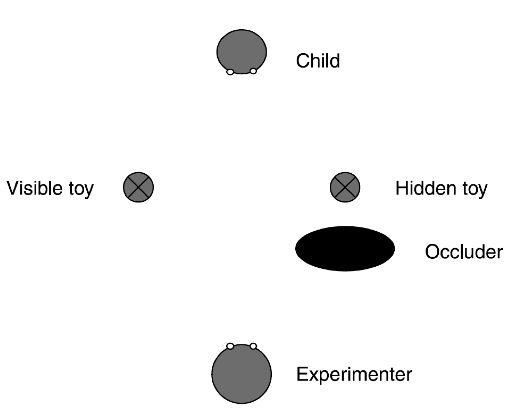
\includegraphics{figure_level_1_perspective_taking.png}
%\caption{
%\label{figure:level_1_perspective_taking}
%Experimental setup for Moll \& Tomasello’s 2006 experiment on level 1 perspective taking.  The experimenter was unable to see one of two objects clearly visible to the child.  When the experimenter asked `I cannot find it! … Can you give it to me?', two-year-olds reliably handed the hidden toy to the experimenter \citep[source: ][figure 1]{en_1202}.
%}
%\end{center}
%\end{figure}
%%
%The authors suggest that children of this age `knew what another person could and could not see when that differed from what they saw'.\footnote{
%	\citet[][p.\ 609]{en_1202}.  
%	Compare \citet[][p.\ 1210]{en_1550} who take subjects' success on a level 1 perspective taking task to show that they
%`could conceptually distinguish what they saw from what another person might see, [and] could think about what the other person saw rather than what they saw when asked to do so.'
%}
%An alternative possibility is that children were representing encountering rather than seeing.  Children may interpret the experimenter’s saying `Where is it? I cannot find it!'\ as expressing an inability to act.  If they also treat having encountered an object as a condition for acting on it, this would explain why they reliably handed the experimenter the object she was not encountering.\footnote{ 	Children in Moll and Tomasello’s experiment reliably work out that the experimenter is requesting something.  This suggests some understanding of pragmatics which could be taken as evidence of much richer theory of mind cognition.  The hypothesis about encountering is neutral on this issue.  Its purpose is only to show that success on these tasks may involve representing encounterings rather than seeings or perceptions.
%}



For another application of the second principle, consider Hare, Call and Tomasello’s finding that chimpanzees reliably adopt strategies which are appropriate given what dominant competitors know about the locations of food \citep[]{en_1545}.  In their `uninformed' condition, a subordinate chimpanzee observed a food item being hidden while a dominant competitor’s view was blocked (see Figure \vref{figure:hare_food_perception}).  In this condition subordinates chose to approach the food significantly more often than in a control condition where the dominant competitor saw the food being hidden.  This indicates that the subordinate chimpanzees were at least indirectly sensitive to facts about what the dominants had perceived.  Several explanations of this finding have already been suggested \citep[]{Call:2008di, en_1551, Suddendorf:2003co}.  A further possibility is that subordinate chimpanzees are aware that the dominant chimpanzee has not encountered the food and take encountering the food to be a condition for the dominant to act with the goal of recovering it.  That would enable them to predict that the subordinate will not be able to retrieve this food in the misinformed condition. 



\begin{figure}
\begin{center}
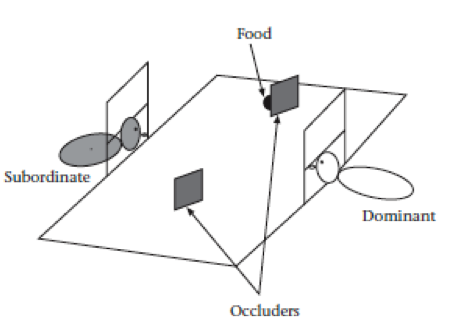
\includegraphics{figure_hare_food_perception.png}
\caption{
	\label{figure:hare_food_perception}
	A subordinate observes as food is placed.  The subordinate can also see the dominant.  There are three conditions: control—the dominant sees food being placed; `uninformed'—the dominant’s view is blocked while the food is placed; and `misinformed'—the dominant sees the food being placed then  has their view blocked while it is moved.
	 \citep[Source:][pp.\ 142, fig. 1]{en_1545}
}
\end{center}
\end{figure}


In short, 
abilities to track others' perceptions  may depend on representing perceptions as such.
But another way to track perceptions would be to represent encounterings and to suppose (as the second principle states) that goal-directed actions involving an object are only possible when the agent has encountered that object.


So far we have been taking for granted that representing encounterings is different from representing perceptions as such.
Why accept this claim? 
It is striking that philosophers have quite different views about what seeing involves—there are debates about whether it is possible to see things without seeing that something is the case \citep[e.g.][]{en_1671}, about whether and in what sense seeing is a representational notion \citep[]{en_1619, en_1705}, and about whether vision is intrinsically a source of knowledge \citep[]{en_1706}, for example.  
There is at least as much uncertainty concerning what might be involved in representing perceptions as such. 
So it is not possible for us to say with certainty what it is to represent perceptions as such.  
Even so, we can be sure that there are some differences between encountering and perception.
If perceptions are representations, then representing perceptions as such plausibly involves representing representations.
Since encounterings are relations not representations (by definition), representing encounterings will  differ from representing perceptions in that only the latter involves representing representations.
But, as mentioned, not everyone agrees that perceptions are representations.
We should therefore consider a bundle of features.
Perception constitutively involves appearances, modalities or the possibility of illusion or is constitutively linked to reasons, knowledge or informational states.
It is plausible that representing perceptions as such involves understanding something about some of these things.
Since encountering does not constitutively involve any of these (by definition), 
representing encounterings may differ from representing perceptions in that it does not require any kind of sensitivity to constitutive links with reasons, knowledge or informational states and nor does it require understanding  anything about appearances, modalities or the possibility of illusion.



\subsection{Third principle}

At this point we switch our attention from conditions on the \textit{occurrence} of goal-directed actions to conditions on their \textit{success}.  Such conditions are more stringent.  Where a goal specifies a particular object, it’s often not enough to have encountered it.  To succeed you must often also have encountered it \textit{in its current location} and to have done so \textit{on your most recent encounter}.  
(There are exceptions, of course.)

We can capture this condition and more by introducing a new notion, \textit{registration}.  Registration is a relation between an individual, an object and a location which will be implicitly defined by principles linking it to encountering and action.  
By design, applying all of these principles would sometimes lead to inconsistencies.  
Where it would be impossible to apply all the principles consistently, consistency is to be achieved by having principles mentioned later trump principles mentioned earlier.
The first  principle defining registration is that an individual registers an object at a location if and only if she most recently encountered it at that location.  As is already clear from this principle, registration is like belief in that it has a correctness condition which may not obtain: a registration is correct when the object is in the location.   Since representing registration brings no benefit for Lucky independently of its connection to action, this principle cannot stand alone in our sequence; it is only the first half of the third principle.

The second half of the third principle states that correct registration is a condition of successful action.  More precisely, in order to successfully perform a goal-directed action with a goal that specifies a particular object, the agent must correctly register that object.%
\footnote{ 	
Some commentators suggested that this principle requires an ability to remember particular encounterings and their temporal order.  There is some evidence that some nonhumans possess this ability \citep[e.g.][]{en_1714, en_1715}, but our proposal does not depend on this.  To track another agent’s most recent encounter, it is not necessary to remember all encounters and their temporal order; forgetting all but the most recent will do.
}  
This principle can be applied in two directions.  In one direction, it licenses Lucky to predict that a competitor who does not have a correct registration of an object will not be successful in performing actions whose goals specify that object.  In the other direction, it allows Lucky, on the basis of observing a successful goal-directed action, to infer that the agent has correctly registered the location of an object.%
\footnote{ 	
The ‘other direction’ is required (in conjunction with the fourth principle, below) for explaining infants’ success on false belief tasks where information about another’s beliefs is provided not by what she sees but by what she does \citep[as in][]{en_1824}.
}
So the principle not only extends Lucky’s ability to predict actions but also her ability to detect what someone registers.  

The correctness of someone’s registrations can be manipulated in their absence by moving or destroying objects they have registered.  So with theory of mind cognition partially characterized by the third principle, Lucky can intentionally prevent others from stealing a food item they have already encountered simply by moving it in their absence.

For an application of this principle, consider Hare, Call and Tomasello’s (\citeyear[]{en_1545}) experiment again.  In a further condition, the `misinformed' condition, a subordinate observer watched as a dominant competitor saw food being hidden.  The subordinate continued to watch as the competitor’s view was blocked and the food moved.  In this case the competitor has encountered the food but does not correctly register it.  
Subordinate observers went for the food more often in this condition than in a control condition where the dominant saw the food being moved.  
This cannot be explained in terms of the second principle.  That principle involved taking encountering an object to be a condition on acting on it.  This condition is met: the competitor \textit{has} encountered the food.  To explain why the subordinate observer goes for the food that has been moved, we need to appeal to the third principle—to correct registration as a condition on success.  It is possible that the subordinate observer realized that the dominant competitor last encountered the food in a location other than its current location.  Suppose the observer also understood that correct registration is a condition on successful goal-directed action.  Then the observer could predict that the competitor would not succeed in retrieving the food.  This could explain why  subordinate observers  more often approach the food in the `misinformed' condition than in the control condition.  

For another application of the third principle, consider scrub-jays who strategically re-cache food depending on who saw what.  In one experiment, scrub-jays cached some food in the presence of Competitor A and then cached more food in the presence of Competitor B.  
Later they had an opportunity to recover food in the presence of Competitor A.  
The scrub-jays preferred to recover and re-cache food cached in the presence of Competitor A, leaving untouched food cached in the presence of the absent competitor \citep[][pp.\ 517-9]{Clayton:2007fh}.  This strategy reduces the chances of Competitor A knowing where any of the scrub-jays’ food is.  What might explain this sensitivity to who saw what in choosing which food to recover?  Clayton and colleagues postulate a capacity to attribute knowledge or `informational states' \citep[]{Clayton:2007fh}.  They are opposed by Penn and colleagues who postulate that scrub-jays are not ascribing knowledge but using rules such as `Try to re-cache food in a site different from the one where it was cached when the competitor was present' \citep[]{en_1417, Penn:2007ey}.  As an alternative to both proposals, the scrub-jays’ sensitivity could be explained in terms of registration.  Suppose scrub-jays understand that correct registration is a condition on successful goal-directed action.  Then they may be trying to prevent competitors from stealing their cached food by means of preventing them from correctly registering its location. 

A third application of the third principle is to infant pointing.  \citet{en_1093} show that 12- and 18-month-olds point in order to provide relevant information to adults about the locations of objects.  In their experiment, infants watch as an adult uses an object in some task.  Then the adult appears to accidentally misplace it.  Later, when the adult visibly needs that object to complete the task again, infants reliably point to it.  Apparently infants point not in order to get the object or to share interest in it, but to enable the adult to complete a task.  The authors suggest that this could be explained either by supposing that infants understand what the adult does not know, or that they understand what the adult is not attending to \citep[][p.\ 185]{en_1093}.  As knowledge and attention are both complex psychological notions, these suggestions raise the hard question of what children might understand of them.  Another possible explanation involves registration.  Maybe the infants understand that correct registration is necessary for successful goal-directed action and that pointing is a way of generating correct registration.  (None of these explanations bear on what is perhaps most interesting about these findings, that infants care to inform others and do so spontaneously.  Minimal theory of mind as described here is at most a small part of a larger story.)

Note that have not argued for the truth of any hypothesis about what chimpanzees, scrub-jays or infants represent.
As explained above, what motivates our enquiry is not that there is already evidence for hypotheses about particular subjects' minimal theory of mind cognition: it is that, given the limited evidence for competing hypotheses and the objections they face, new hypotheses are worth formulating and testing.
And in later sections we will explain how hypotheses about minimal theory of mind generate testable predictions, enabling them to be empirically distinguished from competing hypotheses.
For now our focus is the question of what a subject could represent that would enable her to track track perceptions, knowledge states and beliefs in ways measured by various experimental paradigms.




\subsection{Fourth principle}

So far Lucky thinks of correct registration as a condition for the success of goal-directed action.  This does not tell her anything about what happens if the condition is not met.  In particular it tells her nothing about how an agent will act when she registers an object incorrectly.  The fourth principle involves a switch from thinking of registration as a success condition to thinking of it as a causal factor.  This principle states that when an agent performs a goal-directed action with a goal that specifies a particular object, the agent will act as if the object were in the location she registers it in.

Now that Lucky understands registration as a factor influencing action it can serve her as a proxy for false belief.  Just as, in a limited but useful range of cases, you can track food sources' toxicities by representing their odours
%, objects’ masses by measuring their weights (within limits) 
and prospective sexual partners’ virtues by representing their plumage, so also you can track beliefs by representing registrations.

Applications of the fourth principle therefore include Onishi and Baillargeon’s (\citeyear[]{en_1092}) false belief task.  Subjects are shown an adult observer who is present while a piece of melon is placed in one box.  In the critical condition, the adult observer is then absent while the melon moves to another box.  Comparative looking times indicate that the subjects, who are 14-month-old infants, expect that the adult will reach into the box not containing the melon.\footnote{ 	This finding is supported by a growing body of related research \citep[including][]{en_1666, en_1690, en_1691, en_1208, en_1261}.}  The authors explain this finding by hypothesizing that the infants are ascribing beliefs about the melon’s location to the adults \citep[][p.\ 257]{en_1092}.  Alternatively, the findings could be explained on the hypothesis that they are tracking registration as a cause of action.


\subsection{Extensions and variations}
With the fourth principle we completed the construction of a minimal theory of mind capable of underwriting success on some false belief tasks.  
We stop here because false belief tasks are often taken to be an acid test for theory of mind.
But of course additonal principles can be added accommodate further theory of mind abilities.  
For instance, further principles might extend the definition of registration.  
Registration was been defined as a relation between agents, objects and locations. 
This definition could be extended to include  other types of property as relata in addition to locations.  
Further notions, such as a relational proxy for tracking desires, could also be added.  
These and other modifications would enable hypotheses about minimal theory of mind cognition  to explain a wider range of theory of mind abilities.%
\footnote{
Infants and two-year-olds' theory of mind abilities involve more than tracking false beliefs about location.
To illustrate, \citet{en_1691} show that infants can use communicated information in predicting actions based on false belief, 
\citet{he:2011_false}  show that 2.5-year-olds can succeed on false belief tasks involving unexpected contents rather than location properties, 
and  \citet{en_1795}  show that 18-month olds are sensitive to inferences that others are likely to make. 
}


Variations on the principles are also possible.  To illustrate, scrub-jays’ caching strategies do not obviously call for an ability to track relations to particular food items: their ultimate aim probably isn’t to prevent others pilfering particular worms but to prevent them from pilfering any worms at all.  Accordingly scrub-jays’ protective caching strategies may involve tracking relations between agents, locations and food types rather than particular objects.  
In general it is possible that there is variation across species in what individuals represent that enables them to track perceptions, knowledge states and beliefs. 
If we attempted to characterise theory of mind cognition using only adult human commonsense psychological notions of perception, knowledge and belief, it would be hard to make systematic  sense of the possibility of such variation.
These commonsense psychological notions are not easy to take apart because they resemble the decision-theoretic notion of expected utility in this respect: they are characterised in part by their roles in a system of explanation \citep{Davidson:1985qg,Davidson:1999ju}.
One virtue of the minimal theory of mind construction is that it enables us to make systematic sense of the possibility of variations. 
%Further enhancements will be needed should their general sensitivity to time and episodes also feature in their theory of mind cognition \citep[see][]{en_1409}.


\subsection{But is it theory of mind cognition?}
The term ‘theory of mind’ has been used in several apparently distinct ways \citep[]{en_1415}.  
On some definitions, all theory of mind cognition involves metarepresentation.\footnote{
See \citet{en_81}.  This view can seem obviously correct if it is assumed that  mental states are all representations.
However, there reasons to doubt this assumption \citep[see, for instance, ][]{Campbell:2002ge}.
}  
Minimal theory of mind involves representing goals to which actions are directed, encounterings and registrations, none of which are are representations. 
So if we accepted this definition, what we have constructed would not count as a form of theory of mind cognition just because no metarepresentation is involved.

On another influential definition, theory of mind cognition begins when subjects ascribe states which function as variables intervening between environmental or behavioural inputs and behavioural outputs, and which play some roles characteristic of mental states (\citealp{en_1416}; \citealp[][p.\ 732]{Penn:2007ey}).  
On this definition, the endpoint in our construction (but no earlier point) does count as theory of mind cognition because registrations are intermediate variables and play a subset of the causal roles characteristic of belief.  
For registrations, like beliefs, are characterised by principles generalising across all goal-directed actions,
can be assigned correctness conditions
and causally influence actions.
(Of course they also differ from beliefs in many ways:
they are not propositional attitudes,  they cannot involve reference to never-existent objects and they are not subject to the norms that arguably characterise belief.)
We use the label ‘minimal theory of mind’ because, relative to this definition, the construction describes a minimally elaborate form of theory of mind cognition,
one that does not the entail cognitive and conceptual demands associated with representing perceptions, knowledge states and beliefs as such  
but is capable of grounding theory of mind abilities that generalise across goal-directed actions and are sufficient for systematic success on some false belief tasks.

In what follows we show that minimal theory of mind cognition has clear signature limits.  These limits generate predictions capable of distinguishing hypotheses about minimal theory of mind both 
	from hypotheses  about  representations of nonintentional behaviour only 
	and also 
	from  hypotheses about full-blown theory of mind cognition. 



\section{Limits: how to distinguish minimal from full-blown theory of mind cognition}
\label{sec:limits1}
How could we distinguish minimal from full-blown theory of mind cognition experimentally?  The point of minimal theory of mind is to enable agents to fake it—that is, to act as if they were reasoning about propositional attitudes, within limits.  Where a task goes beyond these limits, we can be sure an agent is not using minimal theory of mind only.

Some limits on minimal theory of mind cognition arise from the fact that the theory makes use of objects and their relations to agents, rather than representations of objects, to predict others’ behaviours.  This means that false beliefs involving quantification or identity cannot be tracked by representing registrations.  To see why not, consider the following inference:
%
\begin{quote}
(1) Mitch believes that Charly is in Baltimore.

(2) Charly is Samantha.

Therefore:

(3) Mitch believes that Samantha is in Baltimore.
\end{quote}
%
On almost any account of belief, this inference is not valid
\citep[][pp.\ 214-5]{frege:1948_sense}.  Its central role in a popular film \citep[]{en_1793} indicates that human adults typically appreciate that this inference is not valid.  Contrast the above inference with the corresponding inference in the case of registration:
%
\begin{quote}
(1$'$) Mitch registers \(<\)Charly, Baltimore\(>\)

(2) Charly is Samantha.

Therefore:

(3$'$) Mitch registers \(<\)Samantha, Baltimore\(>\)
\end{quote}
%
This inference from (1$'$) and (2) to (3$'$) is logically valid.  It is valid because registration is a relation to objects.  We can compare registration with other relations like being left of something.  If Charly is Samantha (whether you know it or not), then anyone who is left of Charly is left of Samantha; similarly for registering Charly’s location. 

This formal difference between belief and registration entails a limit on minimal theory of mind cognition.  Consider Lucky who tracks beliefs by means of representing registrations only and is unable to represent beliefs. Lucky should have no problem predicting actions based on false beliefs about the locations of objects but she should encounter difficulties in predicting actions based on beliefs essentially involving mistakes about identity.  In particular, Lucky should not be able to understand why, when Mitch registers \(<\)Charly, Baltimore\(>\), he continues searching for Samantha.\footnote{ 	This assumes that Lucky herself knows that Charly is Samantha.  To ease exposition we assume throughout that Lucky has no false beliefs involving identity.}  For to register \(<\)Charly, Baltimore\(>\) is the same thing as registering \(<\)Samantha, Baltimore\(>\). And Lucky should be equally at a loss when those she observes mistakenly believe that two distinct people are identical.  By contrast, subjects who can represent beliefs as such should have no special problem with false beliefs essentially involving identity.  This is how mistakes about the identities of objects can be used to distinguish minimal from full-blown theory of mind cognition.%
\footnote{ 	
Related points about quantification entail further testable distinctions.  For instance, minimal theory of mind should make it impossible to track beliefs whose contents essentially involve \textit{most} objects having a certain property.  It is beyond the scope of this paper to elaborate on these predictions.
}

How could this be exploited experimentally?  One paradigm suitable for infants would involve a puppet which has a concave face and body so that,  unusually, it looks very different when seen from different angles.  Viewed from one angle, the puppet looks like one person (Charly); viewed from another angle, the puppet looks like another person (Samantha); and viewed head-on both aspects of its appearance become visible simultaneously.  Crucially, it is possible to see either aspect without having reason to suppose that the puppet would look so different from another angle.  Subjects sit at a table opposite the protagonist.   There is a screen in the middle of the table which blocks each person’s view of the other side of the table.  In the critical condition, the puppet is initially on the subjects’ side of the screen (see Figure \vref{figure:charlie_samantha_experiment}).  In the first scene, the puppet emerges from the screen so that both observers can see it.  Only one aspect of the puppet is revealed to each; the protagonist sees the Charly-aspect, the subject sees the other aspect.  In the second scene the puppet returns to the subjects’ side of the screen; she then rotates.  The subject but not the protagonist is thereby shown that the face and body have two aspects.  Finally, in scene three, the puppet emerges from the screen.  The puppet again reveals only one aspect of its face and body to each observer but this time the protagonist sees the Samantha-aspect and the subject sees the other aspect.  At this point the puppet leaves the stage altogether. Subjects can see that there is nothing on their side of screen, but the protagonist cannot see this. 
Critically, this means that there is reason for the  protagonist to expect there still to be a puppet (Charly) behind the screen.  
So when, finally, the protagonist reaches around the screen, this action makes sense:
	though there is actually nothing behind the screen, the protagonist has reason to expect there is a puppet.
But for subjects to appreciate that the protagonist has this expectation, and to make sense of her reaching action, they would have to ascribe a false belief about identity.%
\footnote{
	To ensure this, the design must be such that subjects cannot readily categorise the puppet’s two appearances and such that subjects do not use verbal labels for the two aspects.  Otherwise it would be possible for subjects to infer the protagonist’s expectation by reasoning about types of object. 
}  
Subjects' lack of surprise at the protagonist's reaching around the screen (as compared to  a control condition which differs from this one only in that the protagonist manifestly knows that the two aspects of the puppet’s face and body are aspects of a single puppet) would therefore be evidence that they can track false beliefs about identity.  
This would be evidence for full-blown, not minimal, theory of mind.


\begin{figure}
\begin{center}
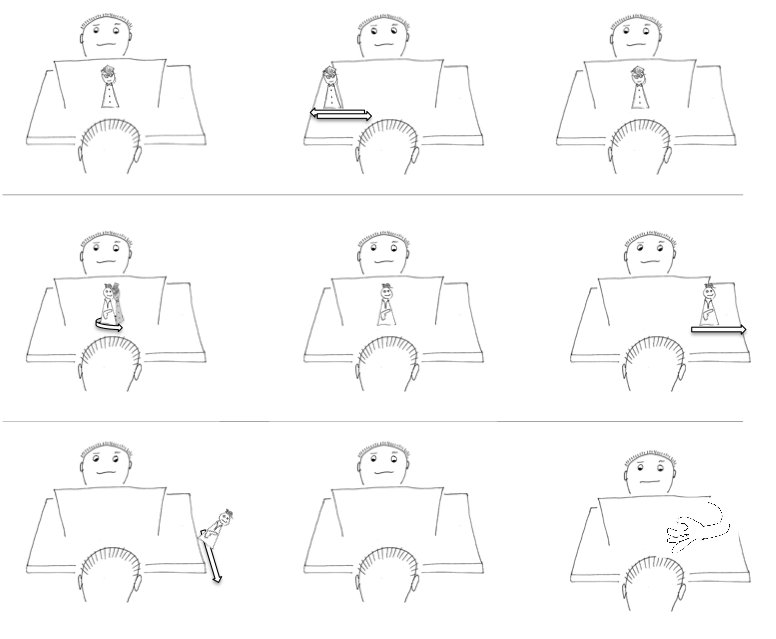
\includegraphics[width=\textwidth]{figure_charlie_samantha_experiment.png}
\caption{
\label{figure:charlie_samantha_experiment}
	How to test whether infants can ascribe false beliefs about identity.  The subject is in the foreground with only the back of  her head visible; the protagonist sits opposite, facing the subject.  A screen conceals some of the action from the protagonist.
}
\end{center}
\end{figure}



So far we have discussed mistaken beliefs about identity where the truth of the belief would require there to be more individuals in the world (Charly and Samantha; a teacher and an assassin) than there actually are.  The converse is also possible \citep[see, e.g.,][]{en_1794}.  Here the mistake is to have beliefs whose truth would require there to be fewer individuals in the world than there actually are. The main condition of a possible experiment is outlined in Figure \vref{figure:identity_balls_experiment}.  In this experiment there are two perceptually indistinguishable balls.  Whereas subjects can see both balls simultaneously, a screen ensures that the protagonist never sees both at once.  The movements of the two balls are timed in such a way that what the protagonist sees indicates the existence of a single ball.%
\footnote{ 	
Song and Baillargeon (\citeyear[]{en_1823}) provide evidence that 15-month-old infants are able to predict actions on the basis of how things appear to observers who are ignorant of their true nature. \citet{en_1822} show that chimpanzees also make inferences about the appearances of things in predicting behaviours. These and other findings \citep[e.g.][]{en_1820} suggest that infants and perhaps others are generally sensitive to facts about the ways things look in tracking others’ beliefs. 
}
When the protagonist sees a ball appear from behind the screen and leave the scene (panels 5-7 in Figure 5), this provides a reason for the protagonist to believe that there is nothing behind the screen.  Infants could only be sensitive to this belief if they were able to track beliefs involving identity.  Sensitivity to this belief might be manifested by comparing this condition with a modified condition in which the protagonist  manifestly knows that there are two balls.  If subjects show more surprise when the protagonist reaches around the screen (say) in the original condition than in the modified condition, this too would be evidence for full-blown over minimal theory of mind cognition.


\begin{figure}
\begin{center}
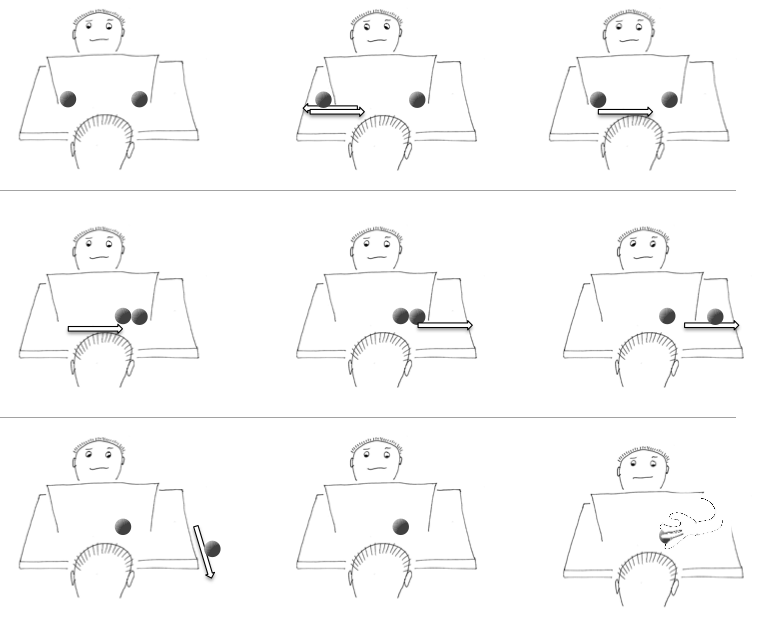
\includegraphics[width=\textwidth]{figure_identity_balls_experiment.png}
\caption{
\label{figure:identity_balls_experiment}
	How to test whether infants can ascribe false beliefs about identity where the mistake involves belief whose truth would entail that there were fewer objects than there in fact are.  As in Figure \ref{figure:charlie_samantha_experiment}, the subject is in the foreground with only the back of  her head visible; the protagonist sits opposite, facing the subject.  A screen conceals some of the action from the protagonist.
}
\end{center}
\end{figure}


Given that this analysis, it is notable that one study already claims to have found positive evidence that infants can ascribe beliefs about identity. 
Scott and Baillargeon (\citeyear{en_1690}) have already conducted experiments which aim to show that 18-month-old infants are able to represent beliefs involving mistakes about `which particular object \textit{token}' another is facing rather than only about `which \textit{type} of object' is present (p.\ 1179). However, while their aim is clearly relevant, we shall show that these experiments do not succeed in testing whether infants ascribe beliefs about identity.  In essence, their paradigm involves two types of object, a divisible penguin which affords hiding a key and an indivisible penguin which lacks this affordance.  The divisible penguin has two states, divided and whole.  When whole it is visually indistinguishable from the indivisible penguin which does not afford hiding a key.  Infants sit opposite a protagonist.  Familiarisation trials provide information that the protagonist can expect there to be two penguins in the scene at all times, one of each type; these trials also provide information that the protagonist can expect the divisible penguin to appear in its divided state. In the critical condition, the scene contains an uncovered and a covered penguin. The uncovered penguin is divisible but, because it is in the whole state, it might easily be taken to be indivisible.  The covered penguin is indivisible.  The findings suggest that infants know that the uncovered penguin is divisible but expect the protagonist to believe that the uncovered penguin is indivisible and to infer that the covered penguin is divisible.  Does this pattern of knowledge and expectation require that the infants have attributed a false belief about identity?  This is not necessary. Suppose that infants attributed the following reasoning to the protagonist: this penguin visible on my right is \textit{an} indivisible penguin; \textit{a} divisible penguin is always present; therefore there is \textit{a} divisible penguin under the cover.  This reasoning concerns only the types of objects present and does not involve identity. Yet it is sufficient (together with some further inferences about the protagonists’ goal) for success. So while Scott and Baillargeon’s (2010) findings are interesting in many respects, their implementation does not provide evidence that infants ascribe beliefs about identity.

In this section we have explained ways of distinguishing minimal theory of mind cognition from its full-blown counterpart.  Where subjects are able to track beliefs about identity we know they are not relying only on minimal theory of mind; and, conversely, where subjects are able to track beliefs about objects’ properties but not about identity, we can infer that they are not using full-blown theory of mind.  We next consider how  minimal theory of mind might be distinguished experimentally from strategies which involve representing nonintentional behaviour only.
	



\section{Limits: how to distinguishing minimal theory of mind from behavioural strategies}
\label{sec:limits2}
What could show that subjects are not solving a task by representing nonintentional behaviour only but are using minimal theory of mind or something stronger?  
We shall use the term ‘behavioural strategy’ to refer to processes underpinning theory of mind abilities which involve representing nonintentional behaviours only. 

An obstacle to distinguishing minimal theory of mind from behavioural strategies is that there is no in-principle limit to the complexity of the predictions which behavioural strategies might support.  The behaviour-representing counterpart of Laplace’s demon knows our entire behavioural histories, has perfect knowledge of the regularities governing object-directed actions and is not limited by scarce cognitive resources.  This demon can readily predict our future behaviours without any theory of mind.  

One way to avoid the problem of the behaviour-representing demon is to set tasks involving explanation rather than prediction \citep[compare][p.\ Chapter 8]{en_167}.  Subjects observe a standard false belief scenario in which a character, Maxi, first searches for an object in the wrong location.  The test question is why Maxi searched as he did \citep[see e.g.][]{en_80, en_352}.  Where subjects’ answers include reference to incorrect registration or a related notion (which might, of course, be verbalised in terms of what an agent ‘thinks’), they have at least minimal theory of mind cognition.  Of course, this only works where subjects can be asked ‘why’ questions.

For other subjects we need an indirect measure.  If subjects sometimes represent encounters or perceptions as such, then representations of others’ encounters may interfere with expectations or judgements about reality or with judgements about one’s own perceptions and beliefs \citep[so-called `altercentric interference',][]{Samson:2010jm}.  For example, representing a protagonists’ encounter with an object at a particular location may interfere with expectations about the object’s actual location.  Accordingly, evidence that there is such interference when in a situation where others have different perceptions or beliefs would provide indirect evidence for theory of mind cognition (minimal or full-blown) over behavioural strategies, for such interference would be difficult to explain if subjects were representing behaviours only. Evidence showing this kind of altercentric interference has recently been found in human adults \citep[]{en_1797, Samson:2010jm}. These studies show that adults’ judgements about the number of objects they could see in a visual scene were slower and more error-prone when the scene contained an irrelevant other whose perspective was different, suggesting that another’s perspective can cause altercentric interfere. 

Of course it was never in question that adults represent encounters or perceptions and not only behaviours; the relevance of these studies is that they demonstrate that altercentric interference can be used as an indirect measure for distinguishing behavioural strategies from minimal theory of mind cognition.  \citet[]{kovacs_social_2010} report evidence of altercentric interference in infants’ expectations about the presence of an object.  Their study suggests that infants’ surprise when their expectations about an object’s presence or absence are violated is modulated by facts about another’s expectations about that object’s location.  Infants looked for less time at the unexpected presence of an object behind a screen when another observer incorrectly expected it to be there than when the observed did not expect it to be there. These findings seem to be evidence of altercentric interference, which is consistent with either minimal or full-blown theory of mind but difficult to explain if participants are exclusively using behavioural strategies.

A related way to distinguish behavioural strategies from minimal theory of mind or something stronger is by means of self-other inference.  Emery and Clayton (\citeyear[]{en_1411}) divided scrub-jays into those who had previously pilfered food and those who had never pilfered.  All subjects then cached some food in private and cached some more food while being observed.  When later given privacy, the pilferers re-cached the food they had earlier cached in the presence of the observer but did not re-cache the food they had cached in private.  The non-pilferers did not show this pattern of behaviour and did little re-caching.\footnote{ 	Similar results might be found if this paradigm were adapted for human infants \citep[see][]{en_1707}.}  This is difficult to reconcile with the hypothesis that scrub-jays rely entirely on behavioural strategies.  By contrast, the hypothesis that scrub-jays have at least minimal theory of mind and so are able to represent goal-directed actions as such allows us to suppose that engaging in pilfering alerts them to the possibility that others may do the same.\footnote{ 	In later discussions these authors claim that the pilferers may be projecting their own experiences onto others in the sense that they are using `their own experiences to infer experiences in others' \citep[][p.\ 81]{Emery:2007ze}.  This claim goes beyond our suggestion, which involves goals rather than experiences and salience rather than projection.  }

Another route to distinguishing minimal theory of mind cognition from behavioural strategies derives from an analogy with speech perception.  It is well established that phoneme recognition is facilitated by lexical information \citep[]{en_1704}.  Similarly, for subjects with (at least) minimal theory of mind cognition, there is evidence that identification of significant segments of behaviour is facilitated by information about goals.  For instance, Zacks (\citeyear[]{en_1442}) varied the availability of information about goals while holding motion features of behaviour constant.  He found that subjects given information about goals segmented behaviour differently from subjects not given such information.  Of course for Zacks it was not in question that his subjects could represent goals; the issue was how their representation of goals interacted with their representations of behaviour.  But with modification the  paradigm could be used to test participants who are not already known to be capable of representing goals.  If making information about goals, encounterings or registrations available alters how subjects segment behaviours, this would be evidence that they are not relying on behavioural strategies only.

In short, a variety of routes to distinguishing behavioural strategies from minimal theory of mind are available.  Some of these involve established paradigms, others adapt ideas from related research.  A decisive argument either way would require converging evidence from multiple paradigms \citep[p.\ 622]{premack_does_1978}.  






\section{Conclusion}

Abilities to track\footnote{
The notion of \emph{tracking} was defined  \vpageref{df:track}; see also the definitions of \emph{theory of mind ability} (\vpageref*{df:tom_ability}) and \emph{theory of mind cognition} (\vpageref*{df:tom_cognition}).
}
perceptions and beliefs are  sometimes but not always  automatic in human adults (or so we argued in Section \ref{sec:motivation}).   
But, as a variety of theoretical and empirical considerations indicate,  representing beliefs and other propositional attitudes as such is associated with demands on working memory, inhibition or attention that are incompatible with automaticity.
This motivated asking what  someone could represent that would enable her to track perceptions, knowledge states and beliefs without meeting these cognitive demands.

Further motivation for asking this question comes from  evidence that theory of mind abilities are widespread, occurring not only in human adults but also in infants, chimpanzees and scrub-jays at least (see Section \ref{sec:more_motivation}).
By contrast full-blown theory of mind cognition may be comparatively rare 
thanks to the conceptual and cognitive demands associated with representing beliefs and other propositional attitudes as such.  
If so it is useful to identify what else someone could represent that would enable her to track, in a limited but useful range of situations, perceptions, knowledge states and beliefs, including false beliefs.  

To answer this question we constructed a minimal theory of mind.  The construction is sufficiently rich to explain systematic success on tasks held to be acid tests for theory of mind cognition including many false belief tasks.  It is also extensible in ways that can explain a range of findings from non-human animals and human infants that are often presented as evidence for full-blown theory of mind cognition.  Where minimal theory of mind must break down is in cases involving quantification or mistakes about identity.  Because such cases require full-blown theory of mind, it is possible to distinguish whether an individual’s performance on a particular task involves minimal or full-blown theory of mind cognition. 

The central notions for minimal theory of mind are encountering and registration.  We characterised these by their structures, acquisition conditions and roles in producing goal-directed actions.  Encountering and registration serve as non-representational proxies for perception and belief in this sense: in a limited but useful range of everyday circumstances, agents perceive an object just when they encounter it and they believe that an object has a given property just when they register it having that property.  But encountering differs from perception in not constitutively involving appearances, modalities or the possibility of illusion and in not being constitutively linked to reasons, knowledge or informational states.  Similarly, registration differs from belief in lacking representational content and the possibility of embedding, in not interacting in arbitrarily complex ways with other states, and in the simplicity of its parameter-setting role in causing actions.  These differences ensure that representing encountering or registration need not involve meeting conceptual and cognitive demands associated with representing perceptions, beliefs and other propositional attitudes as such.

The novelty of our constructive approach lies in several features.  It does not rely directly on everyday psychological concepts, whose exact nature is a source of controversy.
Nor does it rely on infants or non-human animals holding theoretical commitment to simplified versions of these concepts (contrast 
	\citealp{en_75};
	\citealp{en_81};
	\citealp{en_2372} and
	\citealp{en_1614}%
).
Importantly, we do not assume that minimal theory of mind develops into full-blown theory of mind in humans.  
It may instead remain distinct, supporting cognitively efficient theory of mind across the lifespan \citep[see][]{Samson:2010jm, en_2397}.  The construction of minimal theory of mind is systematic enough to generate testable predictions distinguishing it from both behavioural stratetgies and full-blown theory of mind cognition (see Sections \ref{sec:limits1} and \ref{sec:limits2}).  
Our construction makes detailed sense of the notion that there are degrees of theory of mind cognition.  
(This is a virtue because while is widely recognised that degrees of theory of mind cognition are needed \citep[e.g.][]{en_610, en_1415}, there have been few detailed attempts to make systematic sense of this possibility.)
It also pushes much further than earlier work the boundaries of what can be achieved without full-blown theory of mind cognition; in particular, it explains how systematic success on a range of false belief tasks (but not those which essentially involve identity or quantification) is possible without representing beliefs or other propositional attitudes as such. Minimal theory of mind may be what enables those with limited cognitive resources or little conceptual sophistication, such as infants, chimpanzees, scrub-jays and human adults under load,  to track  perceptions, knowledge states and beliefs. 


















\small
\bibliography{$HOME/endnote/phd_biblio_en_record_num_keys}

\end{document}